\section{Introduction}
\label{intro}
Location-based services are becoming more and more essential today, we start to get used to arranging a weekend trip by searching on Yelp for highly rated places, or finding a satisfying restaurant nearby on Foursquare at unfamiliar places. For better usage of the POIs existed on the map, one of the most important information about a POI is the category it belongs to, without which it couldn't be reached by users who haven't been there before. For example, Figure \ref{fig:vivo} showed a map from google with several POIs, in the case that we are in this area and wish to find electronic shop, we'd better know ``Best Denki'' is a electronic retailer, which unfortunately not labeled in the map. Thus our problem is to automatically classify POIs on the map into different categories. In this paper we use global classification hierarchy from Foursquare as standard categories, for example ``Best Denki'' will be first classified as ``Shop \& Service'', which is a first level category, and then further classified as ``Electronics Store'', which is a second level category. Global categories are more welcomed in providing the fullest possible list for general requests, otherwise users may wonder if there are some other qualified candidates with a different label in an ad-hoc label system, for example the labels maybe restaurant, buffet, caf��, burger joint, pizza place, which all belongs to ``Food''.
\begin{figure}[ht]
% Use the relevant command to insert your figure file.
% For example, with the graphicx package use
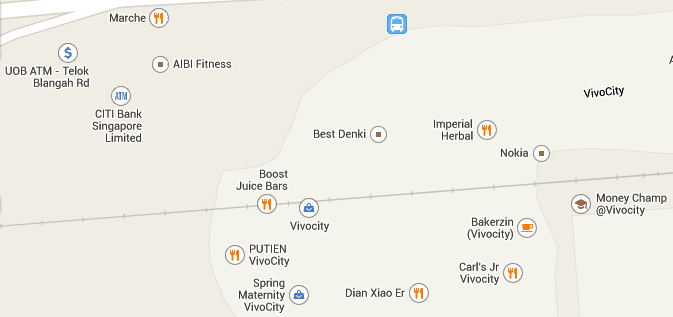
\includegraphics[width=\columnwidth, natwidth = 500, natheight = 230]{VenueGraph/vivocity.PNG}
%  \epsfig{file=VenueGraph/vivocityrec.eps,width=\columnwidth}
% figure caption is below the figure
\caption{Vivocity, Singapore (from Google map)}
\label{fig:vivo}       % Give a unique label
\end{figure}

Obviously, we are not completely blind when facing an uncategorized POI. Some information born with a POI, such as its name, users' check-in record, and the location of the POI. We think these information essential for a POI, and consider them as the only resource we got in our problem. There are many clues in inferring what category a place belongs to based on these information. Intuitively, there can be features extracted directly from the POI's name.  And the most well-studied clue would be user check-in activities. Ye.et al.\cite{yemao} first formulated the problem as a multi-label classification problem and proposed to tackle it by building a binary classifier for each tag, i.e. category in our problem, which we followed in this paper. They introduced some features based on statistical analysis, including population features(e.g., number of a POI's total check-ins) and temporal features(e.g. 24-hour distribution of check-in time). We find these features very effective, and we use them as BASE features to start with. As for our work, we go on adding features generated from the POI's location, and prove them being effective. Some other works introduced other resources including audio clips from smartphone\cite{smartphone}, and user trajectories to help in annotate a POI. These resources are not as common as the information we required in our problem. They are difficult to obtain and not open to public, thus limits their application. There are also some interesting work \cite{userbehavior} on analyzing user's check-in behavior though these features not intended to classify POIs, which focus more on statistical analysis of user behavior rather than discriminating features for classifying POIs.

\begin{figure}[ht]
\begin{minipage}[ht]{0.49\linewidth}
\centering
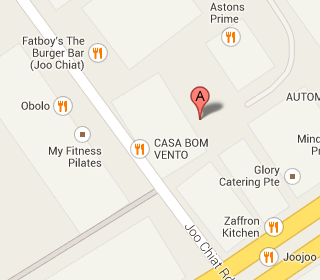
\includegraphics[width=\columnwidth,natwidth = 240, natheight= 230]{VenueGraph/CasaBomVento.PNG}
\caption{Casa Bom Vento, Singapore (from Google map)}
\label{fig:EgCasa}
\end{minipage}
\begin{minipage}[ht]{0.51\linewidth}
\centering
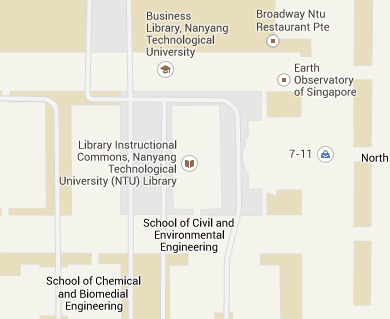
\includegraphics[width=\columnwidth,natwidth = 310, natheight= 239]{VenueGraph/ntu.PNG}
\caption{NTU, Singapore (from Google map)}
\label{fig:EgNTU}
\end{minipage}
\end{figure}

During our exploration on this problem, we find an interesting aspect of POI that is helpful, compensates name features and user behavior features, and yields good result as well: spatial information. The POIs near each other won't necessarily indicate same category indeed, however the location of a POI is definitely far from being a random choice but a deliberate selection, which deeply influenced by the category of the POI and the neighbors around the POI. Therefore, spatial features help in a different angle other than name features and user behavior features. Take a not so popular restaurant with only one user and one check-in record in our data in Sinagpore for example, as shown in Figure \ref{fig:EgCasa}. The restaurant's name is ``Casa Bom Vento'', which is a very opaque name thus leaving name features useless. Neither name features or check-in statistic features can help in predicting its category. But according to the spatial analysis, the fact that the POI is surrounded by restaurants adds probability of the POI belonging to category ``Food''. Therefore, with spatial information, we conclude ``Casa Bom Vento'' more probable belongs to ``Food''. In addition to POI with same categories gathering together as shown in Figure \ref{fig:EgCasa}, POIs with same category tend to have similar neighborhood, for example restaurant and shopping malls are often near each other as shown in Figure \ref{fig:vivo}, and schools and libraries are gathering together as shown in \ref{fig:EgNTU} . Apart from above, POIs with same category having similar spatial conditions is also possible, for example ski parks are often quite alone by themselves.

On the other hand, it appears that although utilizing user behavior is effective, digging it too hard won't necessarily gain better result on POI classification. The reasons are as following. Firstly, normal users' check-in frequency is insufficient to make a reasonable profile of a user's visiting interest, thus no convincing connections between POIs visited by the same user. Active users there might be, but we can't count on there are active users for all uncategorized POIs. Secondly, unlike movie or music, where users' behavior depend mostly on users' interest, the check-in routine of an individual user will only partly be influenced by user's interest, and probably more by normal life, e.g. working place, shopping place, or restaurant. But without differentiation of user's interest and normal life, connections between the places introduced by individual users would be too noisy for classifying POIs. In other words, the main difference between POI in different categories is not who the users that visit them are, but how the users visit them. That's why we found statistics over large amount of users, such as 24-hour check-in distribution, and 7-day check-in distribution, effective. However the relatedness score inferred from user-place relationship from Ye. et al's work can not help to classify on our data. Thus, in our work, we use only Ye et al's statistic features as BASE, not including the inferred scores.


In this paper, we focus on exploring spatial information of POI and extracting descriptive features for POI classification. We first prove several spatial characteristics exists, then propose ways to extract features based on the characteristics. Not only the POI's relative distances with each other are carefully analyzed, comparisons of user behavior between POIs with spatial relations are also included. Then we show their effectiveness by the ability to improve classification results, given the fact that name features and check-in statistics features already yield good results.


According to our observation on spatial characteristics and verification on their effectiveness, we propose four kinds of spatial features, including analysis on location alone, for example nearest K POIs, and comparing user behavior with other POIs within certain distance. These features share some overlap while showing different strength in classifying different categories. We will discuss such difference and tune combinations of features to select best one for each category. We do experiments on second level categories, which are more specified, and show stable advantage over baseline.
Our work has made several contributions as listed below.
\begin{itemize}
\item We exploit POIs relative location and combining with check-in records and analyze several spatial characteristics among different kinds of POIs.

\item  We prove spatial features are individually descriptive and effective, then we choose the best combination for each category and we outperformed baseline of name features and check-in features in experiment on real data from Foursquare.
\end{itemize}
